\documentclass{article}
\usepackage[utf8]{inputenc}
\usepackage{graphicx}

\title{Network of Favors in P2P cloud federation}
\author{Gustavo Diniz Monteiro \\ \href{gustavo.monteiro@ccc.ufcg.edu.br, gustavo.d.monteiro@icloud.com} }
\date{November 2018}


\begin{document}

\maketitle

\section{Modality}

This work will follow the project portfolio modality and aims to implement a previously described concept of Network of Favors\cite{nof}, focusing on aspects of software engineering and the platform usability.

\paragraph{Mentor:} Francisco Vilar Brasileiro

\section{Abstract}
Many organizations have extreme fluctuations of use, and during these peaks, they have to resort to public clouds to meet fleeting demand. The cost of such an action in itself can be expensive, which together with possible sub-utilization of the resources belonging to the organization can generates high costs. The objective of this work is to present a way of implantation and incentive justice on resources sharing in P2P systems, initially using the direct reciprocity model called Network of Favors. The model that will be used for small and medium-sized networks, for scenarios where repeated peer interaction is most likely and where these organizations could meet their demand at peak times and offer favors in under utilization, with guarantee of protection against uncooperative members. In addition, the network focuses on being a lightweight solution and designed to be a pluggable and adaptable element to the provider, using first-hand knowledge gained by each member through direct interaction with other peers.

\section{The Problem}
Organizations with varying demand patterns and utilization peaks often resort to public clouds to meet unexpected or short-term needs, thus escaping failures in meeting business demands and quality of service goals.
However, outside of peak times, the resources belonging to these organizations may become inactive, which is a loss of efficiency.

Under these circumstances, selling these surplus resources may be an interesting option for large private cloud providers, but not for smaller private providers.

One alternative that small and medium-sized private cloud providers may find advantageous is to collaboratively exchange idle capacity on a peer-to-peer (P2P) basis within a federation. In this case, each provider in the federation acts both as a resource provider (outside peak hours) and as a resource consumer (during peak times). In particular private cloud providers, because of the usually limited amount of own resources, would benefit greatly from this exchange, thus allowing them to access a larger pool of resources when local demand is too high and can not be met using only local resources and resources that simply do not exist locally.

\section{Objectives}
The objective of this work is the implementation of a system that allows the creation of a network of favors, which works as a guarantor of justice, and that will work in a connectable way, giving generous support to different federation providers through specific connection modules for each provider, who will act as adapters, and following one of the justice algorithms for favors networks, also implemented as modules, so that the system is configurable and adaptable to the model of justice and to the federation provider of those who propose to use it, as follows in the following architecture diagram.

\begin{center}
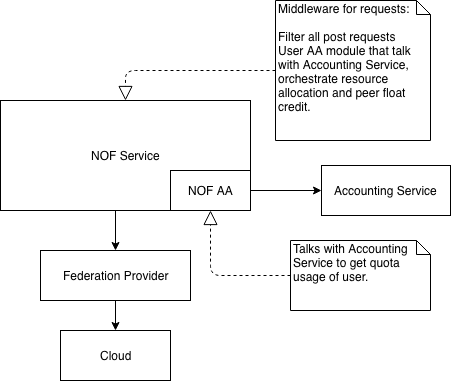
\includegraphics[scale=0.4]{./image/NOF-architecture-generic.png}
\end{center}

\section{Schedule}

The development of this study is planned to take place between January and June of the referent year of 2019 and will be divided into 3 main stages:

\begin{center}
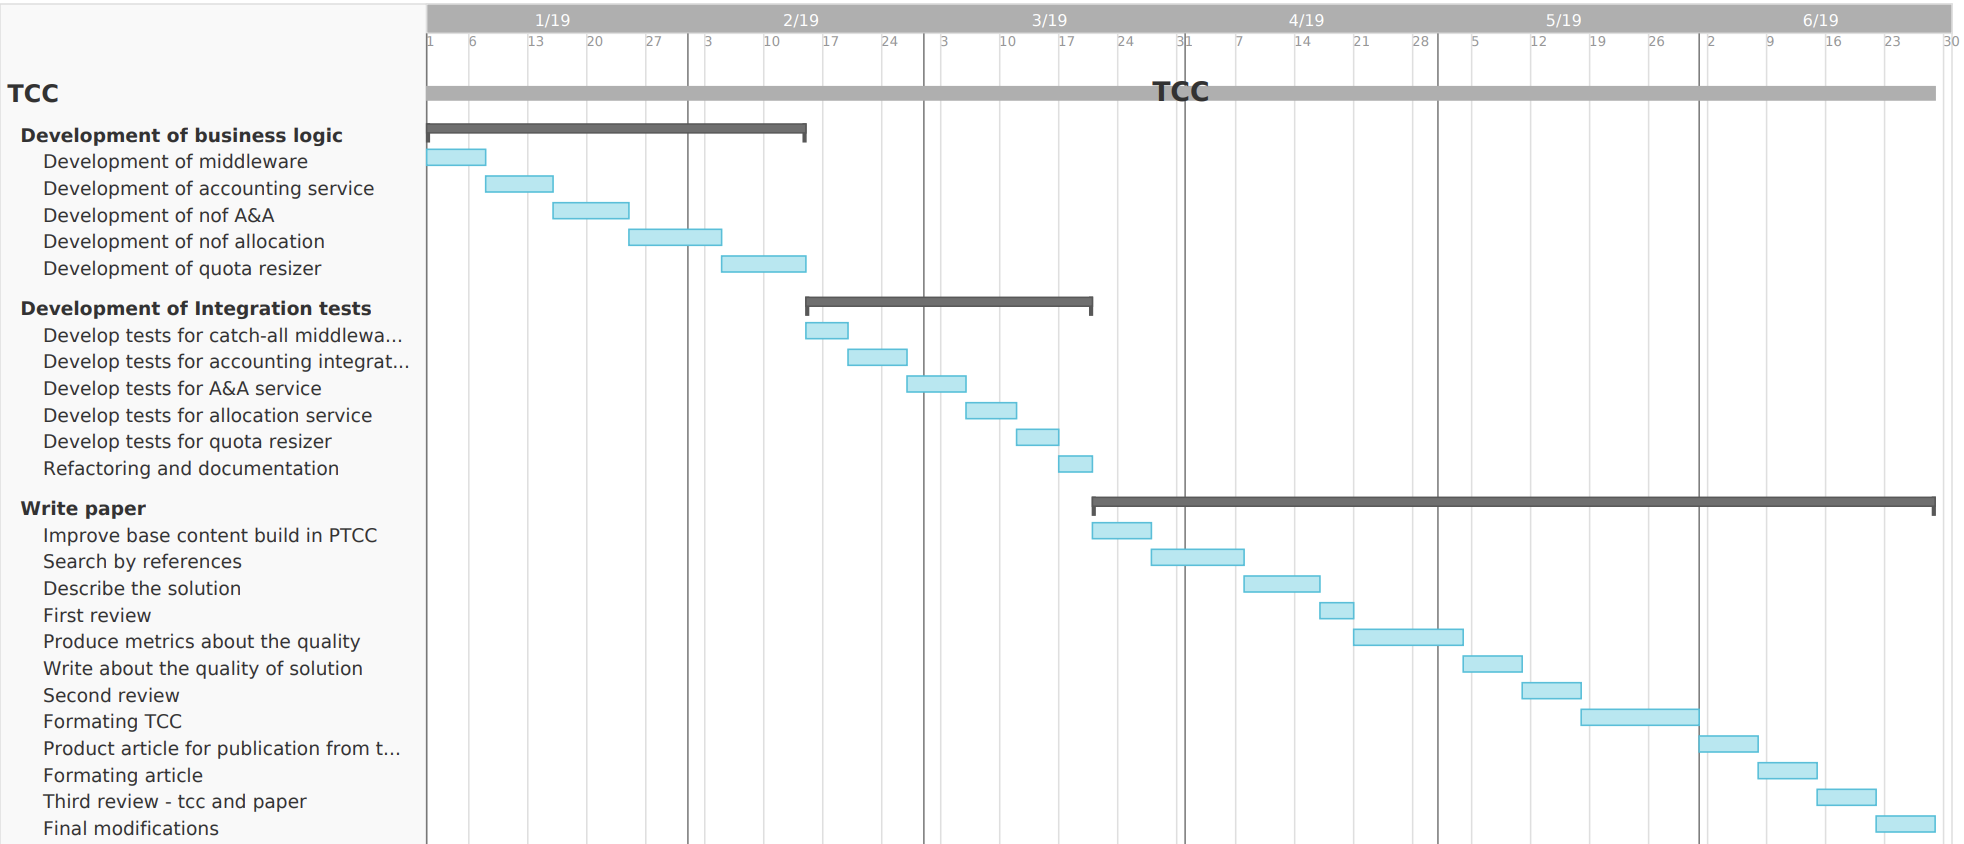
\includegraphics[scale=0.35]{./image/TCC-schedule.png}
\end{center}

\subsection{Development of application business logic}
	In the initial phase, the interfaces and the standard implementation of the components that address the business logic of the NOF service, including the requisition middleware, federation authentication service and favour accounting service, will be developed, in addition to constructing the flows the allocation of requisitions and the scaling of quotas, responsible for the implementation of justice, in parallel will be developed unit tests related to its components. The scheduled time for this activity is during the months of January and February.
\subsection{Development of integration tests}
    In this step, the integration tests of the tool of the NOF component with the tool of provisioning and administration of federations of Fogbow hybrid clouds will be developed. Integration testing will be developed to test all of the most common streams of resource requests, Fogbow sourcing, special non-member member detection cases, and resiliency in cases of error. The deadline for this activity is to do so throughout the month of March.
\subsection{Write the paper}
    This last phase will be dedicated to the writing of the article, where all the decisions of software engineering and re results obtained with the NOF tool will be discussed for this work, which includes all the revisions of the article and possible revisions of architecture and / or implementation in the NOF it was planned to take 3 months, from April to June.

\begin{thebibliography}{9}
\bibitem{nof} 
N. Andrade, F. Brasileiro, W. Cirne, and M. Mowbray, “Automatic grid
assembly by promoting collaboration in peer-to-peer grids,” Journal of
Parallel and Distributed Computing, vol. 67, no. 8, pp. 957 – 966, 2007.
\end{thebibliography}
    
\end{document}